\documentclass[tikz,border=2pt]{standalone}
\usepackage{amsmath,amssymb}
\usepackage{tikz}
\usetikzlibrary{arrows.meta,calc,positioning}

\begin{document}
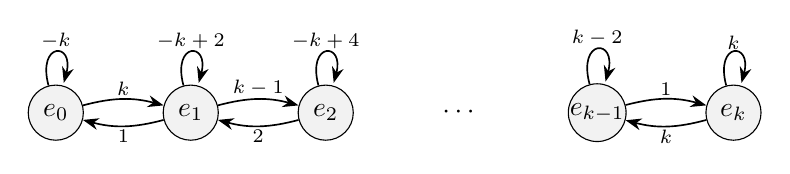
\begin{tikzpicture}[>=Stealth, node distance=1cm]
  % --- Unified styles (all circles same size) ---
    \tikzset{
      vtx/.style     = {circle,draw,fill=gray!10,inner sep=0pt,minimum size=7mm},
      vtxEnd/.style  = {circle,draw,fill=gray!25,inner sep=0pt,minimum size=7mm},
      Ek/.style      = {->,line width=.6pt},          % right arrows
      Fk/.style      = {->,line width=.6pt},          % left arrows
      Hk/.style      = {->,line width=.6pt,looseness=5,min distance=3mm}, % smaller self-loops
      lab/.style     = {font=\scriptsize, inner sep=1pt}
    }

    % --- Basis nodes e_0,...,e_k (endpoints slightly darker but same size) ---
    \node[vtx] (e0) {$e_0$};
    \node[vtx,right=of e0] (e1) {$e_1$};
    \node[vtx,right=of e1] (e2) {$e_2$};
    \node[right=of e2] (dots2) {$\cdots$};
    \node[vtx,right=of dots2] (ekm1) {$e_{k-1}$};
    \node[vtx,right=of ekm1] (ek) {$e_k$};

    % --- Rightward arrows (E_k action): labels are just the coefficients ---
    \draw[Ek] (e0)   to[bend left=15] node[lab,above] {$k$}      (e1);
    \draw[Ek] (e1)   to[bend left=15] node[lab,above] {$k-1$}    (e2);
    \draw[Ek] (ekm1) to[bend left=15] node[lab,above] {$1$}      (ek);

    % --- Leftward arrows (F_k action): labels are just the coefficients ---
    \draw[Fk] (e1)  to[bend left=15] node[lab,below] {$1$}    (e0);
    \draw[Fk] (e2) to[bend left=15] node[lab,below] {$2$}  (e1);
    \draw[Fk] (ek)  to[bend left=15] node[lab,below] {$k$}    (ekm1);

    % --- Self-loops (H_k eigenvalues): labels are just the values ---
    \draw[Hk] (e0) edge[loop above] node[lab] {$-k$} (e0);
    \draw[Hk] (e1) edge[loop above] node[lab] {$-k+2$} (e1);
    \draw[Hk] (e2) edge[loop above] node[lab] {$-k+4$} (e2);
    \draw[Hk] (ekm1) edge[loop above] node[lab] {$k-2$} (ekm1);
    \draw[Hk] (ek) edge[loop above] node[lab] {$k$} (ek);

\end{tikzpicture}
\end{document}
